\documentclass[twoside]{book}

% Packages required by doxygen
\usepackage{fixltx2e}
\usepackage{calc}
\usepackage{doxygen}
\usepackage[export]{adjustbox} % also loads graphicx
\usepackage{graphicx}
\usepackage[utf8]{inputenc}
\usepackage{makeidx}
\usepackage{multicol}
\usepackage{multirow}
\PassOptionsToPackage{warn}{textcomp}
\usepackage{textcomp}
\usepackage[nointegrals]{wasysym}
\usepackage[table]{xcolor}

% Font selection
\usepackage[T1]{fontenc}
\usepackage[scaled=.90]{helvet}
\usepackage{courier}
\usepackage{amssymb}
\usepackage{sectsty}
\renewcommand{\familydefault}{\sfdefault}
\allsectionsfont{%
  \fontseries{bc}\selectfont%
  \color{darkgray}%
}
\renewcommand{\DoxyLabelFont}{%
  \fontseries{bc}\selectfont%
  \color{darkgray}%
}
\newcommand{\+}{\discretionary{\mbox{\scriptsize$\hookleftarrow$}}{}{}}

% Page & text layout
\usepackage{geometry}
\geometry{%
  a4paper,%
  top=2.5cm,%
  bottom=2.5cm,%
  left=2.5cm,%
  right=2.5cm%
}
\tolerance=750
\hfuzz=15pt
\hbadness=750
\setlength{\emergencystretch}{15pt}
\setlength{\parindent}{0cm}
\setlength{\parskip}{3ex plus 2ex minus 2ex}
\makeatletter
\renewcommand{\paragraph}{%
  \@startsection{paragraph}{4}{0ex}{-1.0ex}{1.0ex}{%
    \normalfont\normalsize\bfseries\SS@parafont%
  }%
}
\renewcommand{\subparagraph}{%
  \@startsection{subparagraph}{5}{0ex}{-1.0ex}{1.0ex}{%
    \normalfont\normalsize\bfseries\SS@subparafont%
  }%
}
\makeatother

% Headers & footers
\usepackage{fancyhdr}
\pagestyle{fancyplain}
\fancyhead[LE]{\fancyplain{}{\bfseries\thepage}}
\fancyhead[CE]{\fancyplain{}{}}
\fancyhead[RE]{\fancyplain{}{\bfseries\leftmark}}
\fancyhead[LO]{\fancyplain{}{\bfseries\rightmark}}
\fancyhead[CO]{\fancyplain{}{}}
\fancyhead[RO]{\fancyplain{}{\bfseries\thepage}}
\fancyfoot[LE]{\fancyplain{}{}}
\fancyfoot[CE]{\fancyplain{}{}}
\fancyfoot[RE]{\fancyplain{}{\bfseries\scriptsize Generated by Doxygen }}
\fancyfoot[LO]{\fancyplain{}{\bfseries\scriptsize Generated by Doxygen }}
\fancyfoot[CO]{\fancyplain{}{}}
\fancyfoot[RO]{\fancyplain{}{}}
\renewcommand{\footrulewidth}{0.4pt}
\renewcommand{\chaptermark}[1]{%
  \markboth{#1}{}%
}
\renewcommand{\sectionmark}[1]{%
  \markright{\thesection\ #1}%
}

% Indices & bibliography
\usepackage{natbib}
\usepackage[titles]{tocloft}
\setcounter{tocdepth}{3}
\setcounter{secnumdepth}{5}
\makeindex

% Hyperlinks (required, but should be loaded last)
\usepackage{ifpdf}
\ifpdf
  \usepackage[pdftex,pagebackref=true]{hyperref}
\else
  \usepackage[ps2pdf,pagebackref=true]{hyperref}
\fi
\hypersetup{%
  colorlinks=true,%
  linkcolor=blue,%
  citecolor=blue,%
  unicode%
}

% Custom commands
\newcommand{\clearemptydoublepage}{%
  \newpage{\pagestyle{empty}\cleardoublepage}%
}

\usepackage{caption}
\captionsetup{labelsep=space,justification=centering,font={bf},singlelinecheck=off,skip=4pt,position=top}

%===== C O N T E N T S =====

\begin{document}

% Titlepage & ToC
\hypersetup{pageanchor=false,
             bookmarksnumbered=true,
             pdfencoding=unicode
            }
\pagenumbering{alph}
\begin{titlepage}
\vspace*{7cm}
\begin{center}%
{\Large A\+R\+C\+A\+DE \\[1ex]\large 1.\+0 }\\
\vspace*{1cm}
{\large Generated by Doxygen 1.8.14}\\
\end{center}
\end{titlepage}
\clearemptydoublepage
\pagenumbering{roman}
\tableofcontents
\clearemptydoublepage
\pagenumbering{arabic}
\hypersetup{pageanchor=true}

%--- Begin generated contents ---
\chapter{Hierarchical Index}
\section{Class Hierarchy}
This inheritance list is sorted roughly, but not completely, alphabetically\+:\begin{DoxyCompactList}
\item \contentsline{section}{Arcade\+Application}{\pageref{class_arcade_application}}{}
\item \contentsline{section}{Arcade\+:\+:Color}{\pageref{struct_arcade_1_1_color}}{}
\item \contentsline{section}{Arcade\+:\+:Core}{\pageref{class_arcade_1_1_core}}{}
\item \contentsline{section}{Arcade\+:\+:I\+A\+Ghost}{\pageref{class_arcade_1_1_i_a_ghost}}{}
\item \contentsline{section}{Arcade\+:\+:I\+Game}{\pageref{class_arcade_1_1_i_game}}{}
\begin{DoxyCompactList}
\item \contentsline{section}{Arcade\+:\+:Pacman}{\pageref{class_arcade_1_1_pacman}}{}
\item \contentsline{section}{Arcade\+:\+:Snake}{\pageref{class_arcade_1_1_snake}}{}
\end{DoxyCompactList}
\item \contentsline{section}{Arcade\+:\+:I\+Library}{\pageref{class_arcade_1_1_i_library}}{}
\begin{DoxyCompactList}
\item \contentsline{section}{Arcade\+:\+:Allegro}{\pageref{class_arcade_1_1_allegro}}{}
\item \contentsline{section}{Arcade\+:\+:Lib\+Caca}{\pageref{class_arcade_1_1_lib_caca}}{}
\item \contentsline{section}{Arcade\+:\+:S\+DL}{\pageref{class_arcade_1_1_s_d_l}}{}
\item \contentsline{section}{Arcade\+:\+:S\+F\+ML}{\pageref{class_arcade_1_1_s_f_m_l}}{}
\end{DoxyCompactList}
\item \contentsline{section}{Arcade\+:\+:I\+Music}{\pageref{class_arcade_1_1_i_music}}{}
\begin{DoxyCompactList}
\item \contentsline{section}{Arcade\+:\+:S\+F\+ML}{\pageref{class_arcade_1_1_s_f_m_l}}{}
\end{DoxyCompactList}
\item \contentsline{section}{Arcade\+:\+:Library\+Loader}{\pageref{class_arcade_1_1_library_loader}}{}
\item \contentsline{section}{Arcade\+:\+:Pixel}{\pageref{struct_arcade_1_1_pixel}}{}
\item \contentsline{section}{Arcade\+:\+:Text}{\pageref{struct_arcade_1_1_text}}{}
\end{DoxyCompactList}

\chapter{Class Index}
\section{Class List}
Here are the classes, structs, unions and interfaces with brief descriptions\+:\begin{DoxyCompactList}
\item\contentsline{section}{\mbox{\hyperlink{class_arcade_1_1_allegro}{Arcade\+::\+Allegro}} }{\pageref{class_arcade_1_1_allegro}}{}
\item\contentsline{section}{\mbox{\hyperlink{class_arcade_application}{Arcade\+Application}} }{\pageref{class_arcade_application}}{}
\item\contentsline{section}{\mbox{\hyperlink{struct_arcade_1_1_color}{Arcade\+::\+Color}} }{\pageref{struct_arcade_1_1_color}}{}
\item\contentsline{section}{\mbox{\hyperlink{class_arcade_1_1_core}{Arcade\+::\+Core}} }{\pageref{class_arcade_1_1_core}}{}
\item\contentsline{section}{\mbox{\hyperlink{class_arcade_1_1_i_a_ghost}{Arcade\+::\+I\+A\+Ghost}} }{\pageref{class_arcade_1_1_i_a_ghost}}{}
\item\contentsline{section}{\mbox{\hyperlink{class_arcade_1_1_i_game}{Arcade\+::\+I\+Game}} }{\pageref{class_arcade_1_1_i_game}}{}
\item\contentsline{section}{\mbox{\hyperlink{class_arcade_1_1_i_library}{Arcade\+::\+I\+Library}} }{\pageref{class_arcade_1_1_i_library}}{}
\item\contentsline{section}{\mbox{\hyperlink{class_arcade_1_1_i_music}{Arcade\+::\+I\+Music}} }{\pageref{class_arcade_1_1_i_music}}{}
\item\contentsline{section}{\mbox{\hyperlink{class_arcade_1_1_lib_caca}{Arcade\+::\+Lib\+Caca}} }{\pageref{class_arcade_1_1_lib_caca}}{}
\item\contentsline{section}{\mbox{\hyperlink{class_arcade_1_1_library_loader}{Arcade\+::\+Library\+Loader}} }{\pageref{class_arcade_1_1_library_loader}}{}
\item\contentsline{section}{\mbox{\hyperlink{class_arcade_1_1_pacman}{Arcade\+::\+Pacman}} }{\pageref{class_arcade_1_1_pacman}}{}
\item\contentsline{section}{\mbox{\hyperlink{struct_arcade_1_1_pixel}{Arcade\+::\+Pixel}} }{\pageref{struct_arcade_1_1_pixel}}{}
\item\contentsline{section}{\mbox{\hyperlink{class_arcade_1_1_s_d_l}{Arcade\+::\+S\+DL}} }{\pageref{class_arcade_1_1_s_d_l}}{}
\item\contentsline{section}{\mbox{\hyperlink{class_arcade_1_1_s_f_m_l}{Arcade\+::\+S\+F\+ML}} }{\pageref{class_arcade_1_1_s_f_m_l}}{}
\item\contentsline{section}{\mbox{\hyperlink{class_arcade_1_1_snake}{Arcade\+::\+Snake}} }{\pageref{class_arcade_1_1_snake}}{}
\item\contentsline{section}{\mbox{\hyperlink{struct_arcade_1_1_text}{Arcade\+::\+Text}} }{\pageref{struct_arcade_1_1_text}}{}
\end{DoxyCompactList}

\chapter{Class Documentation}
\hypertarget{class_arcade_1_1_allegro}{}\section{Arcade\+:\+:Allegro Class Reference}
\label{class_arcade_1_1_allegro}\index{Arcade\+::\+Allegro@{Arcade\+::\+Allegro}}
Inheritance diagram for Arcade\+:\+:Allegro\+:\begin{figure}[H]
\begin{center}
\leavevmode
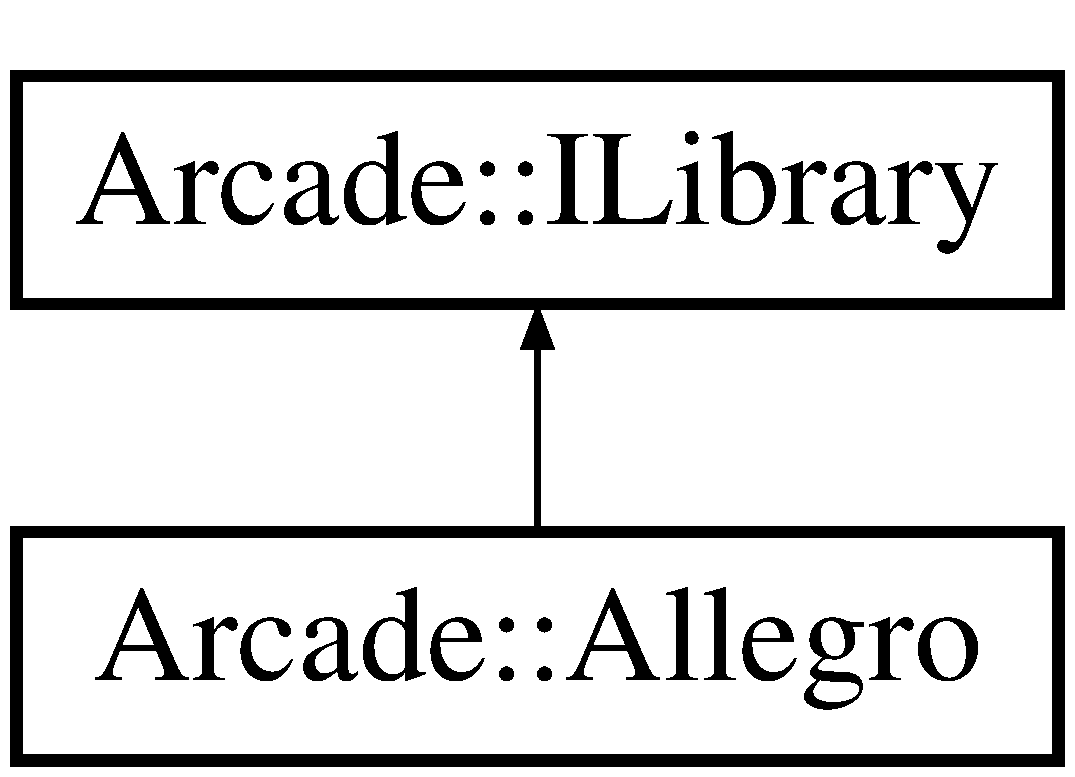
\includegraphics[height=2.000000cm]{class_arcade_1_1_allegro}
\end{center}
\end{figure}
\subsection*{Public Member Functions}
\begin{DoxyCompactItemize}
\item 
\mbox{\Hypertarget{class_arcade_1_1_allegro_ad9b199f394b561e6e2c5a7c010d4e594}\label{class_arcade_1_1_allegro_ad9b199f394b561e6e2c5a7c010d4e594}} 
void {\bfseries create\+Window} ()
\item 
\mbox{\Hypertarget{class_arcade_1_1_allegro_a7e02624a95c302739bd0782e96b84693}\label{class_arcade_1_1_allegro_a7e02624a95c302739bd0782e96b84693}} 
void {\bfseries destroy\+Window} ()
\item 
\mbox{\Hypertarget{class_arcade_1_1_allegro_a01c39163297a7c7aeb35b0755a7de018}\label{class_arcade_1_1_allegro_a01c39163297a7c7aeb35b0755a7de018}} 
Arcade\+::\+Input {\bfseries get\+Input} ()
\item 
\mbox{\Hypertarget{class_arcade_1_1_allegro_a1c43b5ab81820516cbebab119663c441}\label{class_arcade_1_1_allegro_a1c43b5ab81820516cbebab119663c441}} 
void {\bfseries put\+Pixel} (\mbox{\hyperlink{struct_arcade_1_1_pixel}{Arcade\+::\+Pixel}} pixel)
\item 
\mbox{\Hypertarget{class_arcade_1_1_allegro_a3366658db0da0594430c284b4a180d41}\label{class_arcade_1_1_allegro_a3366658db0da0594430c284b4a180d41}} 
void {\bfseries put\+Text} (const \mbox{\hyperlink{struct_arcade_1_1_text}{Arcade\+::\+Text}} \&text)
\item 
\mbox{\Hypertarget{class_arcade_1_1_allegro_a7437f5e92431f00ef1a8017894197d1f}\label{class_arcade_1_1_allegro_a7437f5e92431f00ef1a8017894197d1f}} 
void {\bfseries draw\+Background} (const std\+::string \&background\+Path)
\item 
\mbox{\Hypertarget{class_arcade_1_1_allegro_a260f5796d4df003735aaf8dad89f21d9}\label{class_arcade_1_1_allegro_a260f5796d4df003735aaf8dad89f21d9}} 
void {\bfseries send\+Score} (unsigned int score)
\item 
\mbox{\Hypertarget{class_arcade_1_1_allegro_a30d1da33c9b8f9c3511b3198efac4423}\label{class_arcade_1_1_allegro_a30d1da33c9b8f9c3511b3198efac4423}} 
void {\bfseries draw\+User\+Interface} ()
\item 
\mbox{\Hypertarget{class_arcade_1_1_allegro_a7317e4d461d8d6b0f5adf4ea66e84374}\label{class_arcade_1_1_allegro_a7317e4d461d8d6b0f5adf4ea66e84374}} 
void {\bfseries send\+Name} (const std\+::string \&name)
\item 
\mbox{\Hypertarget{class_arcade_1_1_allegro_aaaefc5e5981661c909eb06e0539370d3}\label{class_arcade_1_1_allegro_aaaefc5e5981661c909eb06e0539370d3}} 
void {\bfseries clear} ()
\item 
\mbox{\Hypertarget{class_arcade_1_1_allegro_a22460ef91180dd139a9d89f6800d79d4}\label{class_arcade_1_1_allegro_a22460ef91180dd139a9d89f6800d79d4}} 
void {\bfseries update} ()
\end{DoxyCompactItemize}


The documentation for this class was generated from the following files\+:\begin{DoxyCompactItemize}
\item 
src/\+Libraries/Allegro.\+hpp\item 
src/\+Libraries/Allegro.\+cpp\end{DoxyCompactItemize}

\hypertarget{class_arcade_application}{}\section{Arcade\+Application Class Reference}
\label{class_arcade_application}\index{Arcade\+Application@{Arcade\+Application}}
\subsection*{Public Member Functions}
\begin{DoxyCompactItemize}
\item 
\mbox{\Hypertarget{class_arcade_application_a00c0b25e8f1d5a5ea1999505983ca6f0}\label{class_arcade_application_a00c0b25e8f1d5a5ea1999505983ca6f0}} 
{\bfseries Arcade\+Application} (int argc, char $\ast$$\ast$argv)
\item 
\mbox{\Hypertarget{class_arcade_application_a76384cdd0e3f9df4aee842a661f311d5}\label{class_arcade_application_a76384cdd0e3f9df4aee842a661f311d5}} 
void {\bfseries launch} ()
\item 
\mbox{\Hypertarget{class_arcade_application_a10c9484628fd182c4caaf9f7da9dc47e}\label{class_arcade_application_a10c9484628fd182c4caaf9f7da9dc47e}} 
void {\bfseries usage} (const char $\ast$program\+Name)
\end{DoxyCompactItemize}


The documentation for this class was generated from the following files\+:\begin{DoxyCompactItemize}
\item 
src/Arcade\+Application.\+hpp\item 
src/Arcade\+Application.\+cpp\end{DoxyCompactItemize}

\hypertarget{struct_arcade_1_1_color}{}\section{Arcade\+:\+:Color Struct Reference}
\label{struct_arcade_1_1_color}\index{Arcade\+::\+Color@{Arcade\+::\+Color}}
\subsection*{Public Member Functions}
\begin{DoxyCompactItemize}
\item 
\mbox{\Hypertarget{struct_arcade_1_1_color_a1df155f54a5207b6d0811a83535c2f21}\label{struct_arcade_1_1_color_a1df155f54a5207b6d0811a83535c2f21}} 
bool {\bfseries operator==} (const \mbox{\hyperlink{struct_arcade_1_1_color}{Arcade\+::\+Color}} \&color) const
\end{DoxyCompactItemize}
\subsection*{Public Attributes}
\begin{DoxyCompactItemize}
\item 
\mbox{\Hypertarget{struct_arcade_1_1_color_a69e890d930f278b9039426696eecb2de}\label{struct_arcade_1_1_color_a69e890d930f278b9039426696eecb2de}} 
unsigned char {\bfseries r}
\item 
\mbox{\Hypertarget{struct_arcade_1_1_color_ad1a83614be521d33f0b9e9a97cd0e8ab}\label{struct_arcade_1_1_color_ad1a83614be521d33f0b9e9a97cd0e8ab}} 
unsigned char {\bfseries g}
\item 
\mbox{\Hypertarget{struct_arcade_1_1_color_a2354b6d3aa07ce9be05fc17214a476e4}\label{struct_arcade_1_1_color_a2354b6d3aa07ce9be05fc17214a476e4}} 
unsigned char {\bfseries b}
\item 
\mbox{\Hypertarget{struct_arcade_1_1_color_ada05b8d7416a374c717ab7780b61359a}\label{struct_arcade_1_1_color_ada05b8d7416a374c717ab7780b61359a}} 
unsigned char {\bfseries a}
\end{DoxyCompactItemize}


The documentation for this struct was generated from the following file\+:\begin{DoxyCompactItemize}
\item 
src/\+Core/Color.\+hpp\end{DoxyCompactItemize}

\hypertarget{class_arcade_1_1_core}{}\section{Arcade\+:\+:Core Class Reference}
\label{class_arcade_1_1_core}\index{Arcade\+::\+Core@{Arcade\+::\+Core}}
\subsection*{Public Member Functions}
\begin{DoxyCompactItemize}
\item 
\mbox{\Hypertarget{class_arcade_1_1_core_ac917342e66c9f5e1ea6debb79a348442}\label{class_arcade_1_1_core_ac917342e66c9f5e1ea6debb79a348442}} 
{\bfseries Core} (std\+::vector$<$ std\+::shared\+\_\+ptr$<$ \mbox{\hyperlink{class_arcade_1_1_i_library}{Arcade\+::\+I\+Library}} $>$$>$ \+\_\+libraries, std\+::vector$<$ std\+::shared\+\_\+ptr$<$ \mbox{\hyperlink{class_arcade_1_1_i_game}{Arcade\+::\+I\+Game}} $>$$>$ \+\_\+games, std\+::shared\+\_\+ptr$<$ \mbox{\hyperlink{class_arcade_1_1_i_music}{Arcade\+::\+I\+Music}} $>$ music\+Library, unsigned int library\+Index)
\item 
\mbox{\Hypertarget{class_arcade_1_1_core_a7996e5cea3d4243c614e68a6557b1c53}\label{class_arcade_1_1_core_a7996e5cea3d4243c614e68a6557b1c53}} 
void {\bfseries core\+Loop} ()
\end{DoxyCompactItemize}


The documentation for this class was generated from the following files\+:\begin{DoxyCompactItemize}
\item 
src/\+Core/Core.\+hpp\item 
src/\+Core/Core.\+cpp\end{DoxyCompactItemize}

\hypertarget{class_arcade_1_1_i_a_ghost}{}\section{Arcade\+:\+:I\+A\+Ghost Class Reference}
\label{class_arcade_1_1_i_a_ghost}\index{Arcade\+::\+I\+A\+Ghost@{Arcade\+::\+I\+A\+Ghost}}
\subsection*{Public Member Functions}
\begin{DoxyCompactItemize}
\item 
\mbox{\Hypertarget{class_arcade_1_1_i_a_ghost_aec64c7bcbaccae0978f3f1c749980540}\label{class_arcade_1_1_i_a_ghost_aec64c7bcbaccae0978f3f1c749980540}} 
{\bfseries I\+A\+Ghost} (\mbox{\hyperlink{struct_arcade_1_1_color}{Color}} color, unsigned int x, unsigned int y, const std\+::string \&path\+Sprite)
\item 
\mbox{\Hypertarget{class_arcade_1_1_i_a_ghost_abc1bab00a21e4aa368a7124a49005e96}\label{class_arcade_1_1_i_a_ghost_abc1bab00a21e4aa368a7124a49005e96}} 
void {\bfseries update} (\mbox{\hyperlink{struct_arcade_1_1_pixel}{Arcade\+::\+Pixel}} player, std\+::vector$<$ \mbox{\hyperlink{struct_arcade_1_1_pixel}{Arcade\+::\+Pixel}} $>$ \&\+\_\+screen, bool eating)
\item 
\mbox{\Hypertarget{class_arcade_1_1_i_a_ghost_a157b76d685a6a3b4627c4ad833ee8a0e}\label{class_arcade_1_1_i_a_ghost_a157b76d685a6a3b4627c4ad833ee8a0e}} 
const \mbox{\hyperlink{struct_arcade_1_1_pixel}{Arcade\+::\+Pixel}} \& {\bfseries get\+Ghost} () const
\item 
\mbox{\Hypertarget{class_arcade_1_1_i_a_ghost_a9602c7b1f04d40bd5989ae4026aba5f6}\label{class_arcade_1_1_i_a_ghost_a9602c7b1f04d40bd5989ae4026aba5f6}} 
void {\bfseries set\+Ghost} (const \mbox{\hyperlink{struct_arcade_1_1_pixel}{Pixel}} \&ghost)
\item 
\mbox{\Hypertarget{class_arcade_1_1_i_a_ghost_ae260a12b6cffefdb188daa1008e0a294}\label{class_arcade_1_1_i_a_ghost_ae260a12b6cffefdb188daa1008e0a294}} 
void {\bfseries set\+Sprite} (const std\+::string \&sprite)
\end{DoxyCompactItemize}


The documentation for this class was generated from the following files\+:\begin{DoxyCompactItemize}
\item 
src/\+Games/\+Pacman/A\+I\+Ghost.\+hpp\item 
src/\+Games/\+Pacman/A\+I\+Ghost.\+cpp\end{DoxyCompactItemize}

\hypertarget{class_arcade_1_1_i_game}{}\section{Arcade\+:\+:I\+Game Class Reference}
\label{class_arcade_1_1_i_game}\index{Arcade\+::\+I\+Game@{Arcade\+::\+I\+Game}}
Inheritance diagram for Arcade\+:\+:I\+Game\+:\begin{figure}[H]
\begin{center}
\leavevmode
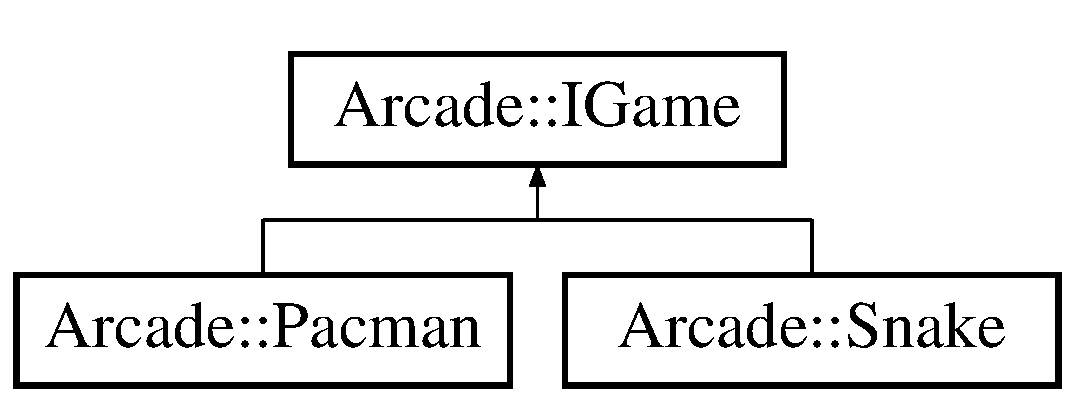
\includegraphics[height=2.000000cm]{class_arcade_1_1_i_game}
\end{center}
\end{figure}
\subsection*{Public Member Functions}
\begin{DoxyCompactItemize}
\item 
\mbox{\Hypertarget{class_arcade_1_1_i_game_ab0b047d4495f483a550bd82e17421474}\label{class_arcade_1_1_i_game_ab0b047d4495f483a550bd82e17421474}} 
virtual std\+::string {\bfseries get\+Name} ()=0
\item 
\mbox{\Hypertarget{class_arcade_1_1_i_game_a00035447a2bc30a5ff302fa1b2ad2cb0}\label{class_arcade_1_1_i_game_a00035447a2bc30a5ff302fa1b2ad2cb0}} 
virtual std\+::vector$<$ std\+::vector$<$ \mbox{\hyperlink{struct_arcade_1_1_pixel}{Arcade\+::\+Pixel}} $>$ $>$ {\bfseries get\+Screen\+Layers} ()=0
\item 
\mbox{\Hypertarget{class_arcade_1_1_i_game_aefab20d9b3b0c511f61a6a7fb7fb42a1}\label{class_arcade_1_1_i_game_aefab20d9b3b0c511f61a6a7fb7fb42a1}} 
virtual std\+::string {\bfseries get\+Background} ()=0
\item 
\mbox{\Hypertarget{class_arcade_1_1_i_game_a8374f492eb8202280408b34b850a9c55}\label{class_arcade_1_1_i_game_a8374f492eb8202280408b34b850a9c55}} 
virtual std\+::string {\bfseries get\+Sound\+Effect} ()=0
\item 
\mbox{\Hypertarget{class_arcade_1_1_i_game_ae68fc6ff4afc8eca2bc34e10aeb58f4e}\label{class_arcade_1_1_i_game_ae68fc6ff4afc8eca2bc34e10aeb58f4e}} 
virtual void {\bfseries send\+Input} (Arcade\+::\+Input input)=0
\item 
\mbox{\Hypertarget{class_arcade_1_1_i_game_a667fc6a62d295e0bcb7b84be03672235}\label{class_arcade_1_1_i_game_a667fc6a62d295e0bcb7b84be03672235}} 
virtual void {\bfseries update} ()=0
\item 
\mbox{\Hypertarget{class_arcade_1_1_i_game_a3f323930377997c179a0d6d806e5f972}\label{class_arcade_1_1_i_game_a3f323930377997c179a0d6d806e5f972}} 
virtual std\+::pair$<$ unsigned int, unsigned int $>$ {\bfseries get\+Res} ()=0
\item 
\mbox{\Hypertarget{class_arcade_1_1_i_game_a81fced9c4187827ce9c763c1d6edc680}\label{class_arcade_1_1_i_game_a81fced9c4187827ce9c763c1d6edc680}} 
virtual unsigned int {\bfseries get\+Score} ()=0
\item 
\mbox{\Hypertarget{class_arcade_1_1_i_game_ac916c384573ea39ad4989ce89797942a}\label{class_arcade_1_1_i_game_ac916c384573ea39ad4989ce89797942a}} 
virtual void {\bfseries reset} ()=0
\end{DoxyCompactItemize}


The documentation for this class was generated from the following file\+:\begin{DoxyCompactItemize}
\item 
src/\+Games/I\+Game.\+hpp\end{DoxyCompactItemize}

\hypertarget{class_arcade_1_1_i_library}{}\section{Arcade\+:\+:I\+Library Class Reference}
\label{class_arcade_1_1_i_library}\index{Arcade\+::\+I\+Library@{Arcade\+::\+I\+Library}}
Inheritance diagram for Arcade\+:\+:I\+Library\+:\begin{figure}[H]
\begin{center}
\leavevmode
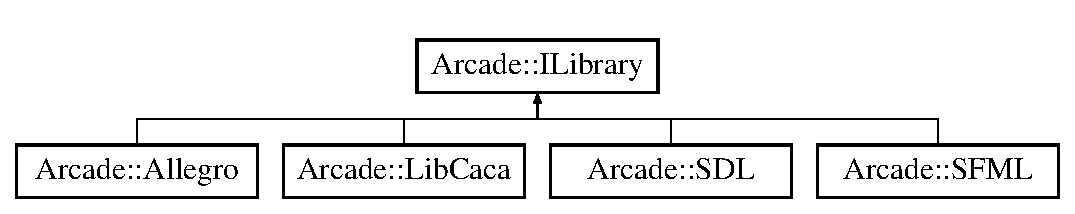
\includegraphics[height=2.000000cm]{class_arcade_1_1_i_library}
\end{center}
\end{figure}
\subsection*{Public Member Functions}
\begin{DoxyCompactItemize}
\item 
\mbox{\Hypertarget{class_arcade_1_1_i_library_a2692a472028ff773b1f5613abf5932f8}\label{class_arcade_1_1_i_library_a2692a472028ff773b1f5613abf5932f8}} 
virtual Arcade\+::\+Input {\bfseries get\+Input} ()=0
\item 
\mbox{\Hypertarget{class_arcade_1_1_i_library_afbc8a084721cd0d0beaa9dbfb8df4c36}\label{class_arcade_1_1_i_library_afbc8a084721cd0d0beaa9dbfb8df4c36}} 
virtual void {\bfseries put\+Pixel} (\mbox{\hyperlink{struct_arcade_1_1_pixel}{Arcade\+::\+Pixel}} pixel)=0
\item 
\mbox{\Hypertarget{class_arcade_1_1_i_library_aa0e372ca4c265215eb52479eafb4ccbf}\label{class_arcade_1_1_i_library_aa0e372ca4c265215eb52479eafb4ccbf}} 
virtual void {\bfseries draw\+Background} (const std\+::string \&background\+Path)=0
\item 
\mbox{\Hypertarget{class_arcade_1_1_i_library_a4c840ecfc867bd7bc6d99a6dc7f08adb}\label{class_arcade_1_1_i_library_a4c840ecfc867bd7bc6d99a6dc7f08adb}} 
virtual void {\bfseries send\+Score} (unsigned int score)=0
\item 
\mbox{\Hypertarget{class_arcade_1_1_i_library_ad71f48b3f2384639b96d8ad1170b19fa}\label{class_arcade_1_1_i_library_ad71f48b3f2384639b96d8ad1170b19fa}} 
virtual void {\bfseries send\+Name} (const std\+::string \&name)=0
\item 
\mbox{\Hypertarget{class_arcade_1_1_i_library_ab93f08e87209f22fb9517f82a040d01a}\label{class_arcade_1_1_i_library_ab93f08e87209f22fb9517f82a040d01a}} 
virtual void {\bfseries draw\+User\+Interface} ()=0
\item 
\mbox{\Hypertarget{class_arcade_1_1_i_library_adfce11518f2243b5414853a9c43bd0ed}\label{class_arcade_1_1_i_library_adfce11518f2243b5414853a9c43bd0ed}} 
virtual void {\bfseries put\+Text} (const \mbox{\hyperlink{struct_arcade_1_1_text}{Arcade\+::\+Text}} \&text)=0
\item 
\mbox{\Hypertarget{class_arcade_1_1_i_library_aec6d25695326978633b64df2748221ba}\label{class_arcade_1_1_i_library_aec6d25695326978633b64df2748221ba}} 
virtual void {\bfseries clear} ()=0
\item 
\mbox{\Hypertarget{class_arcade_1_1_i_library_a165b072a1e4c29b70954f3236d418426}\label{class_arcade_1_1_i_library_a165b072a1e4c29b70954f3236d418426}} 
virtual void {\bfseries update} ()=0
\item 
\mbox{\Hypertarget{class_arcade_1_1_i_library_a9841d65f5411d231971ead51575ac81c}\label{class_arcade_1_1_i_library_a9841d65f5411d231971ead51575ac81c}} 
virtual void {\bfseries create\+Window} ()=0
\item 
\mbox{\Hypertarget{class_arcade_1_1_i_library_af6d9d01fea85b8dae789836ad20d2388}\label{class_arcade_1_1_i_library_af6d9d01fea85b8dae789836ad20d2388}} 
virtual void {\bfseries destroy\+Window} ()=0
\end{DoxyCompactItemize}


The documentation for this class was generated from the following file\+:\begin{DoxyCompactItemize}
\item 
src/\+Libraries/I\+Library.\+hpp\end{DoxyCompactItemize}

\hypertarget{class_arcade_1_1_i_music}{}\section{Arcade\+:\+:I\+Music Class Reference}
\label{class_arcade_1_1_i_music}\index{Arcade\+::\+I\+Music@{Arcade\+::\+I\+Music}}
Inheritance diagram for Arcade\+:\+:I\+Music\+:\begin{figure}[H]
\begin{center}
\leavevmode
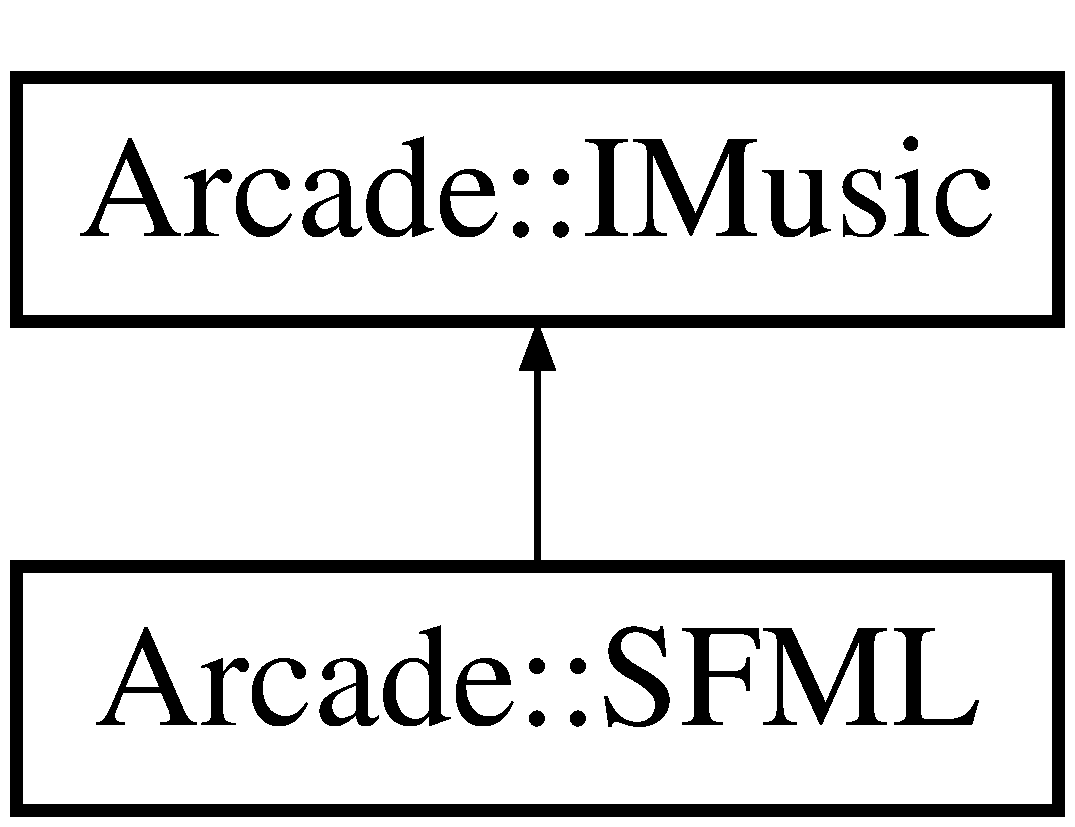
\includegraphics[height=2.000000cm]{class_arcade_1_1_i_music}
\end{center}
\end{figure}
\subsection*{Public Member Functions}
\begin{DoxyCompactItemize}
\item 
\mbox{\Hypertarget{class_arcade_1_1_i_music_a12467cea18f1d76fd2d7ff9725ea9f11}\label{class_arcade_1_1_i_music_a12467cea18f1d76fd2d7ff9725ea9f11}} 
virtual void {\bfseries play\+Sound} (const std\+::string \&path, bool loop, float volume)=0
\item 
\mbox{\Hypertarget{class_arcade_1_1_i_music_a7c58da4b2c4396e878dc90ee0820bbcb}\label{class_arcade_1_1_i_music_a7c58da4b2c4396e878dc90ee0820bbcb}} 
virtual void {\bfseries clean\+Sounds} ()=0
\end{DoxyCompactItemize}


The documentation for this class was generated from the following file\+:\begin{DoxyCompactItemize}
\item 
src/\+Libraries/I\+Music.\+hpp\end{DoxyCompactItemize}

\hypertarget{class_arcade_1_1_lib_caca}{}\section{Arcade\+:\+:Lib\+Caca Class Reference}
\label{class_arcade_1_1_lib_caca}\index{Arcade\+::\+Lib\+Caca@{Arcade\+::\+Lib\+Caca}}
Inheritance diagram for Arcade\+:\+:Lib\+Caca\+:\begin{figure}[H]
\begin{center}
\leavevmode
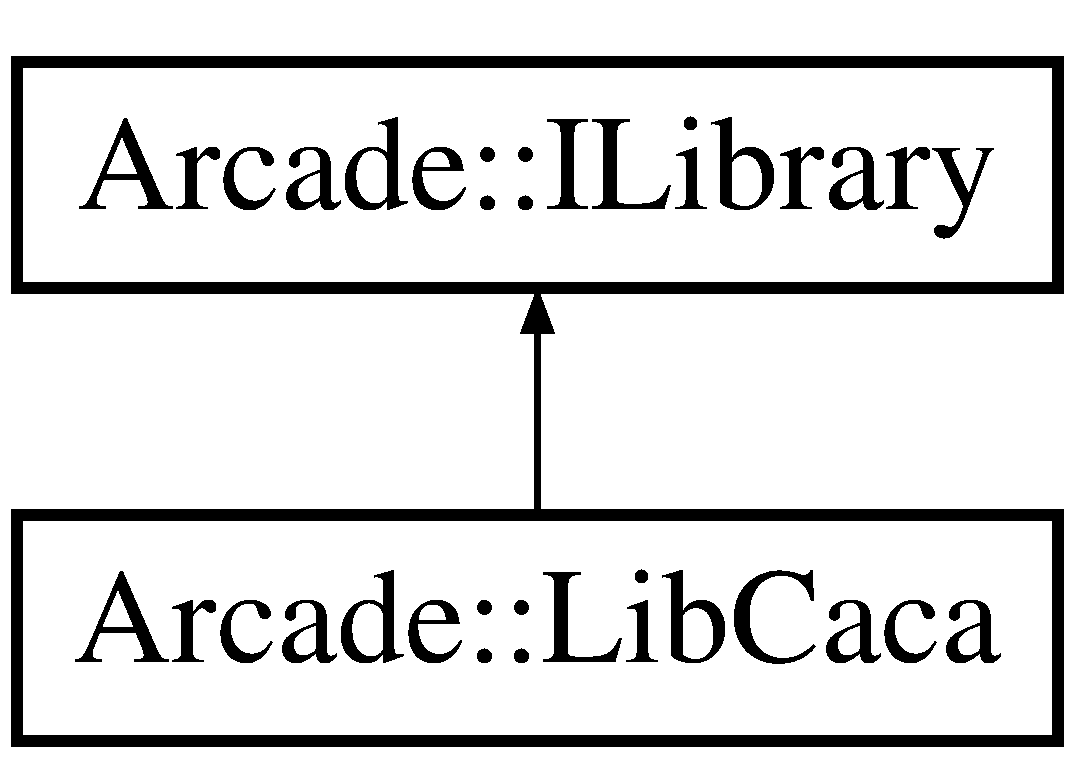
\includegraphics[height=2.000000cm]{class_arcade_1_1_lib_caca}
\end{center}
\end{figure}
\subsection*{Public Member Functions}
\begin{DoxyCompactItemize}
\item 
\mbox{\Hypertarget{class_arcade_1_1_lib_caca_ae3918f8b4ecc275f0cbd807197050b9a}\label{class_arcade_1_1_lib_caca_ae3918f8b4ecc275f0cbd807197050b9a}} 
void {\bfseries create\+Window} ()
\item 
\mbox{\Hypertarget{class_arcade_1_1_lib_caca_a825f6c9c47d466cc4fed08495c790bbe}\label{class_arcade_1_1_lib_caca_a825f6c9c47d466cc4fed08495c790bbe}} 
void {\bfseries destroy\+Window} ()
\item 
\mbox{\Hypertarget{class_arcade_1_1_lib_caca_ae8b2aeeeb8657f1dfacab3f68f9bdf01}\label{class_arcade_1_1_lib_caca_ae8b2aeeeb8657f1dfacab3f68f9bdf01}} 
Arcade\+::\+Input {\bfseries get\+Input} ()
\item 
\mbox{\Hypertarget{class_arcade_1_1_lib_caca_af582e74761b4356b77222373763637e1}\label{class_arcade_1_1_lib_caca_af582e74761b4356b77222373763637e1}} 
void {\bfseries put\+Pixel} (\mbox{\hyperlink{struct_arcade_1_1_pixel}{Arcade\+::\+Pixel}} pixel)
\item 
\mbox{\Hypertarget{class_arcade_1_1_lib_caca_a75e72a37708be917094c7701f3a3efb6}\label{class_arcade_1_1_lib_caca_a75e72a37708be917094c7701f3a3efb6}} 
void {\bfseries put\+Text} (const \mbox{\hyperlink{struct_arcade_1_1_text}{Arcade\+::\+Text}} \&text)
\item 
\mbox{\Hypertarget{class_arcade_1_1_lib_caca_aebd4f7b7b1cef143dfd689a9ef7fb4f4}\label{class_arcade_1_1_lib_caca_aebd4f7b7b1cef143dfd689a9ef7fb4f4}} 
void {\bfseries draw\+Background} (const std\+::string \&background\+Path)
\item 
\mbox{\Hypertarget{class_arcade_1_1_lib_caca_a59ef9475b8d22b35f654513d2958d49d}\label{class_arcade_1_1_lib_caca_a59ef9475b8d22b35f654513d2958d49d}} 
void {\bfseries send\+Score} (unsigned int score)
\item 
\mbox{\Hypertarget{class_arcade_1_1_lib_caca_ab0fbaae32c1e17acba24e9bedea8331b}\label{class_arcade_1_1_lib_caca_ab0fbaae32c1e17acba24e9bedea8331b}} 
void {\bfseries draw\+User\+Interface} ()
\item 
\mbox{\Hypertarget{class_arcade_1_1_lib_caca_aeab911efbbf909329191a89afeed9d29}\label{class_arcade_1_1_lib_caca_aeab911efbbf909329191a89afeed9d29}} 
void {\bfseries send\+Name} (const std\+::string \&name)
\item 
\mbox{\Hypertarget{class_arcade_1_1_lib_caca_afa5402ae9cda10be3aa4ef167dc9d515}\label{class_arcade_1_1_lib_caca_afa5402ae9cda10be3aa4ef167dc9d515}} 
void {\bfseries clear} ()
\item 
\mbox{\Hypertarget{class_arcade_1_1_lib_caca_ad050187725b650516bb3841d0a4a0fea}\label{class_arcade_1_1_lib_caca_ad050187725b650516bb3841d0a4a0fea}} 
void {\bfseries update} ()
\end{DoxyCompactItemize}


The documentation for this class was generated from the following files\+:\begin{DoxyCompactItemize}
\item 
src/\+Libraries/Lib\+Caca.\+hpp\item 
src/\+Libraries/Lib\+Caca.\+cpp\end{DoxyCompactItemize}

\hypertarget{class_arcade_1_1_library_loader}{}\section{Arcade\+:\+:Library\+Loader Class Reference}
\label{class_arcade_1_1_library_loader}\index{Arcade\+::\+Library\+Loader@{Arcade\+::\+Library\+Loader}}
\subsection*{Public Member Functions}
\begin{DoxyCompactItemize}
\item 
\mbox{\Hypertarget{class_arcade_1_1_library_loader_a86c84394fa12f14b4f23f9e1d0bbb932}\label{class_arcade_1_1_library_loader_a86c84394fa12f14b4f23f9e1d0bbb932}} 
void $\ast$ {\bfseries load\+Library} (std\+::string library\+Path)
\item 
\mbox{\Hypertarget{class_arcade_1_1_library_loader_afca7cd7281b961989434b65717da8c36}\label{class_arcade_1_1_library_loader_afca7cd7281b961989434b65717da8c36}} 
void $\ast$ {\bfseries get\+Function} (void $\ast$handle, std\+::string function\+Name)
\item 
\mbox{\Hypertarget{class_arcade_1_1_library_loader_a6f10513581d8bc548bc7032ccd139adb}\label{class_arcade_1_1_library_loader_a6f10513581d8bc548bc7032ccd139adb}} 
void {\bfseries close\+Library} (void $\ast$handle)
\item 
\mbox{\Hypertarget{class_arcade_1_1_library_loader_ab05b9e050ece987db0d4409b1ba55069}\label{class_arcade_1_1_library_loader_ab05b9e050ece987db0d4409b1ba55069}} 
bool {\bfseries is\+Library\+Of\+Type} (void $\ast$handle, const std\+::string \&type)
\end{DoxyCompactItemize}


The documentation for this class was generated from the following files\+:\begin{DoxyCompactItemize}
\item 
src/Library\+Loader.\+hpp\item 
src/Library\+Loader.\+cpp\end{DoxyCompactItemize}

\hypertarget{class_arcade_1_1_pacman}{}\section{Arcade\+:\+:Pacman Class Reference}
\label{class_arcade_1_1_pacman}\index{Arcade\+::\+Pacman@{Arcade\+::\+Pacman}}
Inheritance diagram for Arcade\+:\+:Pacman\+:\begin{figure}[H]
\begin{center}
\leavevmode
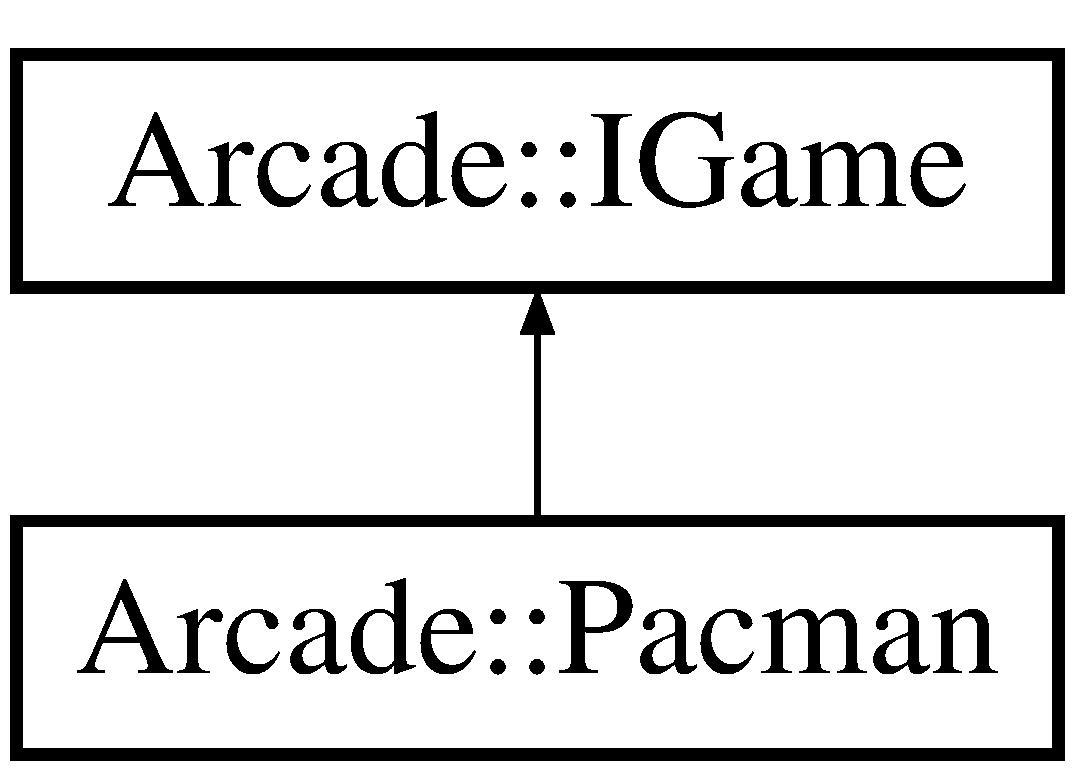
\includegraphics[height=2.000000cm]{class_arcade_1_1_pacman}
\end{center}
\end{figure}
\subsection*{Public Member Functions}
\begin{DoxyCompactItemize}
\item 
\mbox{\Hypertarget{class_arcade_1_1_pacman_ae94a4c324525be0937af7bd6c326194b}\label{class_arcade_1_1_pacman_ae94a4c324525be0937af7bd6c326194b}} 
std\+::string {\bfseries get\+Name} ()
\item 
\mbox{\Hypertarget{class_arcade_1_1_pacman_a8ce3e1d50b4003f8ceca30eb9a15d311}\label{class_arcade_1_1_pacman_a8ce3e1d50b4003f8ceca30eb9a15d311}} 
std\+::vector$<$ std\+::vector$<$ \mbox{\hyperlink{struct_arcade_1_1_pixel}{Arcade\+::\+Pixel}} $>$ $>$ {\bfseries get\+Screen\+Layers} () override
\item 
\mbox{\Hypertarget{class_arcade_1_1_pacman_ae911e033a81ef3ad0178cd1303b9e2df}\label{class_arcade_1_1_pacman_ae911e033a81ef3ad0178cd1303b9e2df}} 
void {\bfseries send\+Input} (Arcade\+::\+Input input) override
\item 
\mbox{\Hypertarget{class_arcade_1_1_pacman_a2e382b9fabef2a49c01fc9ee52de34f1}\label{class_arcade_1_1_pacman_a2e382b9fabef2a49c01fc9ee52de34f1}} 
void {\bfseries update} () override
\item 
\mbox{\Hypertarget{class_arcade_1_1_pacman_afd65d2a017ada9379f4f76e3b99c9c54}\label{class_arcade_1_1_pacman_afd65d2a017ada9379f4f76e3b99c9c54}} 
std\+::pair$<$ unsigned int, unsigned int $>$ {\bfseries get\+Res} ()
\item 
\mbox{\Hypertarget{class_arcade_1_1_pacman_af21245973ba39b98b7f8cc18b23d1abc}\label{class_arcade_1_1_pacman_af21245973ba39b98b7f8cc18b23d1abc}} 
unsigned int {\bfseries get\+Score} ()
\item 
\mbox{\Hypertarget{class_arcade_1_1_pacman_aa2c7a7a0c05c99e23906a4a4196ddb7b}\label{class_arcade_1_1_pacman_aa2c7a7a0c05c99e23906a4a4196ddb7b}} 
std\+::string {\bfseries get\+Background} ()
\item 
\mbox{\Hypertarget{class_arcade_1_1_pacman_ae40b68b5eb83a1d4528169c357129f67}\label{class_arcade_1_1_pacman_ae40b68b5eb83a1d4528169c357129f67}} 
bool {\bfseries is\+Eating} () const
\item 
\mbox{\Hypertarget{class_arcade_1_1_pacman_af4a4bcc2f50e28a785a33bc37a915388}\label{class_arcade_1_1_pacman_af4a4bcc2f50e28a785a33bc37a915388}} 
void {\bfseries reset} () override
\item 
\mbox{\Hypertarget{class_arcade_1_1_pacman_a6dfb2aa4cef6c1f3d79895aaa0e5b6c8}\label{class_arcade_1_1_pacman_a6dfb2aa4cef6c1f3d79895aaa0e5b6c8}} 
std\+::string {\bfseries get\+Sound\+Effect} () override
\end{DoxyCompactItemize}


The documentation for this class was generated from the following files\+:\begin{DoxyCompactItemize}
\item 
src/\+Games/\+Pacman/Pacman.\+hpp\item 
src/\+Games/\+Pacman/Pacman.\+cpp\end{DoxyCompactItemize}

\hypertarget{struct_arcade_1_1_pixel}{}\section{Arcade\+:\+:Pixel Struct Reference}
\label{struct_arcade_1_1_pixel}\index{Arcade\+::\+Pixel@{Arcade\+::\+Pixel}}
\subsection*{Public Attributes}
\begin{DoxyCompactItemize}
\item 
\mbox{\Hypertarget{struct_arcade_1_1_pixel_a2ed5805b28213cf913de41e0a5c34603}\label{struct_arcade_1_1_pixel_a2ed5805b28213cf913de41e0a5c34603}} 
unsigned int {\bfseries x}
\item 
\mbox{\Hypertarget{struct_arcade_1_1_pixel_a507eb7771cecce88d4d5b3235296835a}\label{struct_arcade_1_1_pixel_a507eb7771cecce88d4d5b3235296835a}} 
unsigned int {\bfseries y}
\item 
\mbox{\Hypertarget{struct_arcade_1_1_pixel_a20c2e376dff38b4b8331e25b06e4efd9}\label{struct_arcade_1_1_pixel_a20c2e376dff38b4b8331e25b06e4efd9}} 
\mbox{\hyperlink{struct_arcade_1_1_color}{Arcade\+::\+Color}} {\bfseries color}
\item 
\mbox{\Hypertarget{struct_arcade_1_1_pixel_a44aadf8b3c8573071670e4d85b6ee1d8}\label{struct_arcade_1_1_pixel_a44aadf8b3c8573071670e4d85b6ee1d8}} 
std\+::string {\bfseries path\+Sprite}
\end{DoxyCompactItemize}


The documentation for this struct was generated from the following file\+:\begin{DoxyCompactItemize}
\item 
src/\+Core/Core.\+hpp\end{DoxyCompactItemize}

\hypertarget{class_arcade_1_1_s_d_l}{}\section{Arcade\+:\+:S\+DL Class Reference}
\label{class_arcade_1_1_s_d_l}\index{Arcade\+::\+S\+DL@{Arcade\+::\+S\+DL}}
Inheritance diagram for Arcade\+:\+:S\+DL\+:\begin{figure}[H]
\begin{center}
\leavevmode
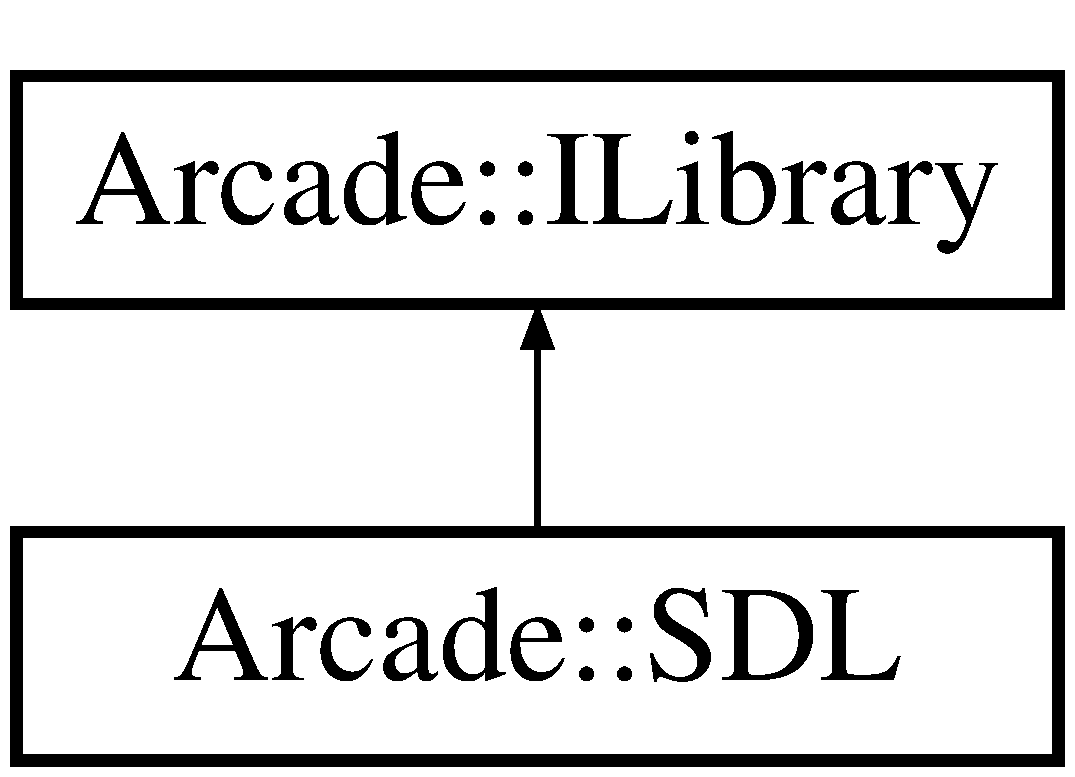
\includegraphics[height=2.000000cm]{class_arcade_1_1_s_d_l}
\end{center}
\end{figure}
\subsection*{Public Member Functions}
\begin{DoxyCompactItemize}
\item 
\mbox{\Hypertarget{class_arcade_1_1_s_d_l_aaef4833a806524b8fb81a69341099c62}\label{class_arcade_1_1_s_d_l_aaef4833a806524b8fb81a69341099c62}} 
void {\bfseries create\+Window} ()
\item 
\mbox{\Hypertarget{class_arcade_1_1_s_d_l_a54eecbeb527daffb86edb09b3116eba5}\label{class_arcade_1_1_s_d_l_a54eecbeb527daffb86edb09b3116eba5}} 
void {\bfseries destroy\+Window} ()
\item 
\mbox{\Hypertarget{class_arcade_1_1_s_d_l_a8e2b64e6963c2c52384954c74ef878dc}\label{class_arcade_1_1_s_d_l_a8e2b64e6963c2c52384954c74ef878dc}} 
Arcade\+::\+Input {\bfseries get\+Input} ()
\item 
\mbox{\Hypertarget{class_arcade_1_1_s_d_l_a80f1de868a87158aedc416ed5af451c1}\label{class_arcade_1_1_s_d_l_a80f1de868a87158aedc416ed5af451c1}} 
void {\bfseries put\+Pixel} (\mbox{\hyperlink{struct_arcade_1_1_pixel}{Arcade\+::\+Pixel}} pixel)
\item 
\mbox{\Hypertarget{class_arcade_1_1_s_d_l_acf96a58981b64e3a41ce1f0adeb65db1}\label{class_arcade_1_1_s_d_l_acf96a58981b64e3a41ce1f0adeb65db1}} 
void {\bfseries put\+Text} (const \mbox{\hyperlink{struct_arcade_1_1_text}{Arcade\+::\+Text}} \&text)
\item 
\mbox{\Hypertarget{class_arcade_1_1_s_d_l_af48b9e73bed971ac6b2713abe120c776}\label{class_arcade_1_1_s_d_l_af48b9e73bed971ac6b2713abe120c776}} 
void {\bfseries draw\+Background} (const std\+::string \&background\+Path)
\item 
\mbox{\Hypertarget{class_arcade_1_1_s_d_l_a6e40941ec661b902aa80acb8fdbbcbf0}\label{class_arcade_1_1_s_d_l_a6e40941ec661b902aa80acb8fdbbcbf0}} 
void {\bfseries send\+Score} (unsigned int score)
\item 
\mbox{\Hypertarget{class_arcade_1_1_s_d_l_aa3470e47c9bd7234ba2ccc4a900cfabe}\label{class_arcade_1_1_s_d_l_aa3470e47c9bd7234ba2ccc4a900cfabe}} 
void {\bfseries draw\+User\+Interface} ()
\item 
\mbox{\Hypertarget{class_arcade_1_1_s_d_l_ada2bee00a245d75e475103cef0e56c66}\label{class_arcade_1_1_s_d_l_ada2bee00a245d75e475103cef0e56c66}} 
void {\bfseries send\+Name} (const std\+::string \&name)
\item 
\mbox{\Hypertarget{class_arcade_1_1_s_d_l_a8635ea8f90f6b70c1af4a550e225e742}\label{class_arcade_1_1_s_d_l_a8635ea8f90f6b70c1af4a550e225e742}} 
void {\bfseries clear} ()
\item 
\mbox{\Hypertarget{class_arcade_1_1_s_d_l_abfceb1c90adb1111eba21c92144e18d2}\label{class_arcade_1_1_s_d_l_abfceb1c90adb1111eba21c92144e18d2}} 
void {\bfseries update} ()
\end{DoxyCompactItemize}


The documentation for this class was generated from the following files\+:\begin{DoxyCompactItemize}
\item 
src/\+Libraries/S\+D\+L.\+hpp\item 
src/\+Libraries/S\+D\+L.\+cpp\end{DoxyCompactItemize}

\hypertarget{class_arcade_1_1_s_f_m_l}{}\section{Arcade\+:\+:S\+F\+ML Class Reference}
\label{class_arcade_1_1_s_f_m_l}\index{Arcade\+::\+S\+F\+ML@{Arcade\+::\+S\+F\+ML}}
Inheritance diagram for Arcade\+:\+:S\+F\+ML\+:\begin{figure}[H]
\begin{center}
\leavevmode
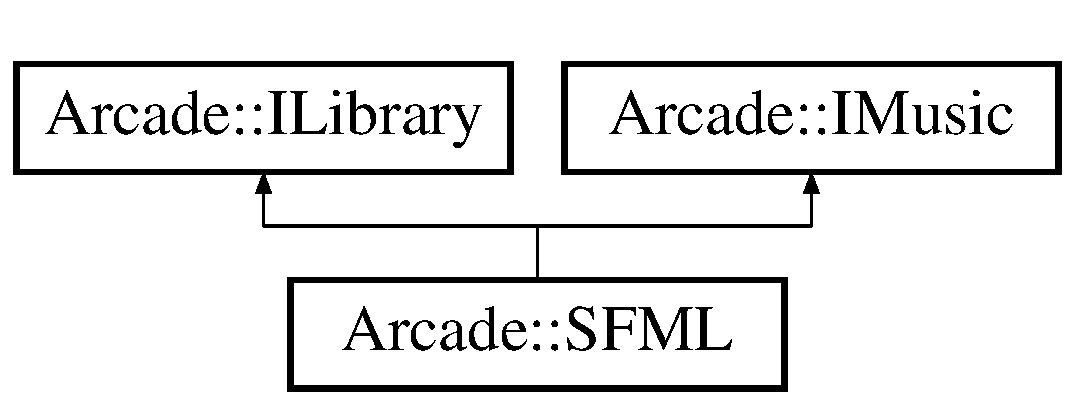
\includegraphics[height=2.000000cm]{class_arcade_1_1_s_f_m_l}
\end{center}
\end{figure}
\subsection*{Public Member Functions}
\begin{DoxyCompactItemize}
\item 
\mbox{\Hypertarget{class_arcade_1_1_s_f_m_l_a3c6dfca064da57299f0a0e4f8ff5d305}\label{class_arcade_1_1_s_f_m_l_a3c6dfca064da57299f0a0e4f8ff5d305}} 
void {\bfseries create\+Window} ()
\item 
\mbox{\Hypertarget{class_arcade_1_1_s_f_m_l_aa08ae3ab8a8217c237ec599e204a24a9}\label{class_arcade_1_1_s_f_m_l_aa08ae3ab8a8217c237ec599e204a24a9}} 
void {\bfseries destroy\+Window} ()
\item 
\mbox{\Hypertarget{class_arcade_1_1_s_f_m_l_aeac5b5148a86cba6a8977f6d117e63e4}\label{class_arcade_1_1_s_f_m_l_aeac5b5148a86cba6a8977f6d117e63e4}} 
Arcade\+::\+Input {\bfseries get\+Input} ()
\item 
\mbox{\Hypertarget{class_arcade_1_1_s_f_m_l_a5ca7ae57f67241a4f5b9ddb0702eaede}\label{class_arcade_1_1_s_f_m_l_a5ca7ae57f67241a4f5b9ddb0702eaede}} 
void {\bfseries put\+Pixel} (\mbox{\hyperlink{struct_arcade_1_1_pixel}{Arcade\+::\+Pixel}} pixel)
\item 
\mbox{\Hypertarget{class_arcade_1_1_s_f_m_l_a3bb920bca7cd72db68d8072889eafab5}\label{class_arcade_1_1_s_f_m_l_a3bb920bca7cd72db68d8072889eafab5}} 
void {\bfseries put\+Text} (const \mbox{\hyperlink{struct_arcade_1_1_text}{Arcade\+::\+Text}} \&text)
\item 
\mbox{\Hypertarget{class_arcade_1_1_s_f_m_l_a9db16260c0ffe79f3e177645fc3a8698}\label{class_arcade_1_1_s_f_m_l_a9db16260c0ffe79f3e177645fc3a8698}} 
void {\bfseries draw\+Background} (const std\+::string \&background\+Path)
\item 
\mbox{\Hypertarget{class_arcade_1_1_s_f_m_l_a7f7b9589ff88722183be1877d870249c}\label{class_arcade_1_1_s_f_m_l_a7f7b9589ff88722183be1877d870249c}} 
void {\bfseries send\+Score} (unsigned int score)
\item 
\mbox{\Hypertarget{class_arcade_1_1_s_f_m_l_ade9704fab4f6a56da66250f29e7a930f}\label{class_arcade_1_1_s_f_m_l_ade9704fab4f6a56da66250f29e7a930f}} 
void {\bfseries draw\+User\+Interface} ()
\item 
\mbox{\Hypertarget{class_arcade_1_1_s_f_m_l_a920d1d15cae228ea47339845f53c01b4}\label{class_arcade_1_1_s_f_m_l_a920d1d15cae228ea47339845f53c01b4}} 
void {\bfseries send\+Name} (const std\+::string \&name)
\item 
\mbox{\Hypertarget{class_arcade_1_1_s_f_m_l_a6c44bbb72121d8f6d5dc510ba0ec89d9}\label{class_arcade_1_1_s_f_m_l_a6c44bbb72121d8f6d5dc510ba0ec89d9}} 
void {\bfseries clear} ()
\item 
\mbox{\Hypertarget{class_arcade_1_1_s_f_m_l_a1f7d18216be0a233c08ab8306d0188f9}\label{class_arcade_1_1_s_f_m_l_a1f7d18216be0a233c08ab8306d0188f9}} 
void {\bfseries update} ()
\item 
\mbox{\Hypertarget{class_arcade_1_1_s_f_m_l_a4edffe9197a038ecc84af72f91976e6d}\label{class_arcade_1_1_s_f_m_l_a4edffe9197a038ecc84af72f91976e6d}} 
void {\bfseries play\+Sound} (const std\+::string \&path, bool loop, float volume)
\item 
\mbox{\Hypertarget{class_arcade_1_1_s_f_m_l_a391fc7d78f675a3d0f88af2b9ec91d12}\label{class_arcade_1_1_s_f_m_l_a391fc7d78f675a3d0f88af2b9ec91d12}} 
void {\bfseries clean\+Sounds} ()
\end{DoxyCompactItemize}


The documentation for this class was generated from the following files\+:\begin{DoxyCompactItemize}
\item 
src/\+Libraries/S\+F\+M\+L.\+hpp\item 
src/\+Libraries/S\+F\+M\+L.\+cpp\end{DoxyCompactItemize}

\hypertarget{class_arcade_1_1_snake}{}\section{Arcade\+:\+:Snake Class Reference}
\label{class_arcade_1_1_snake}\index{Arcade\+::\+Snake@{Arcade\+::\+Snake}}
Inheritance diagram for Arcade\+:\+:Snake\+:\begin{figure}[H]
\begin{center}
\leavevmode
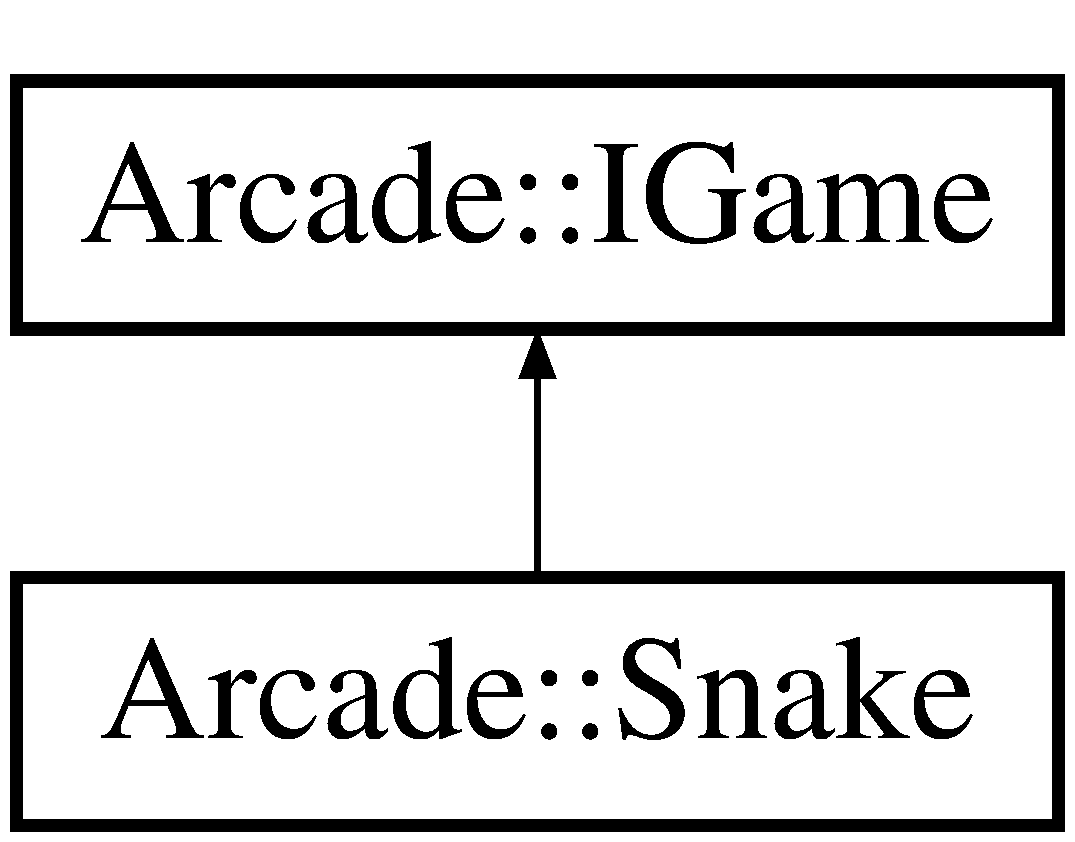
\includegraphics[height=2.000000cm]{class_arcade_1_1_snake}
\end{center}
\end{figure}
\subsection*{Public Member Functions}
\begin{DoxyCompactItemize}
\item 
\mbox{\Hypertarget{class_arcade_1_1_snake_a81d76742b5f390319bb383eae69e5b35}\label{class_arcade_1_1_snake_a81d76742b5f390319bb383eae69e5b35}} 
std\+::string {\bfseries get\+Name} () override
\item 
\mbox{\Hypertarget{class_arcade_1_1_snake_a2244b7ddff8a96595b08b4d32c91ae1a}\label{class_arcade_1_1_snake_a2244b7ddff8a96595b08b4d32c91ae1a}} 
std\+::vector$<$ std\+::vector$<$ \mbox{\hyperlink{struct_arcade_1_1_pixel}{Arcade\+::\+Pixel}} $>$ $>$ {\bfseries get\+Screen\+Layers} () override
\item 
\mbox{\Hypertarget{class_arcade_1_1_snake_a97f904344bad3695d6308d8c79f3ae3f}\label{class_arcade_1_1_snake_a97f904344bad3695d6308d8c79f3ae3f}} 
std\+::string {\bfseries get\+Background} () override
\item 
\mbox{\Hypertarget{class_arcade_1_1_snake_a739564b0409e6c7f812fe3d10d40bcc6}\label{class_arcade_1_1_snake_a739564b0409e6c7f812fe3d10d40bcc6}} 
void {\bfseries send\+Input} (Arcade\+::\+Input input) override
\item 
\mbox{\Hypertarget{class_arcade_1_1_snake_a609165f1482aed55cf891faf9882a543}\label{class_arcade_1_1_snake_a609165f1482aed55cf891faf9882a543}} 
void {\bfseries update} () override
\item 
\mbox{\Hypertarget{class_arcade_1_1_snake_a25900c449009a252291ac105e6b6a8f2}\label{class_arcade_1_1_snake_a25900c449009a252291ac105e6b6a8f2}} 
std\+::pair$<$ unsigned int, unsigned int $>$ {\bfseries get\+Res} () override
\item 
\mbox{\Hypertarget{class_arcade_1_1_snake_a39d0275ab08feadd2a470427aae4ac95}\label{class_arcade_1_1_snake_a39d0275ab08feadd2a470427aae4ac95}} 
unsigned int {\bfseries get\+Score} () override
\item 
\mbox{\Hypertarget{class_arcade_1_1_snake_aaffec5fc20dd354d6d23aa422c9e8e43}\label{class_arcade_1_1_snake_aaffec5fc20dd354d6d23aa422c9e8e43}} 
void {\bfseries pop\+Fruit} ()
\item 
\mbox{\Hypertarget{class_arcade_1_1_snake_a75067f8baf7687b4d8561e3d2fb2a8e7}\label{class_arcade_1_1_snake_a75067f8baf7687b4d8561e3d2fb2a8e7}} 
bool {\bfseries check\+Snake} (\mbox{\hyperlink{struct_arcade_1_1_pixel}{Arcade\+::\+Pixel}} target)
\item 
\mbox{\Hypertarget{class_arcade_1_1_snake_aae0d4d9d12da29a8bc34010d077c9f53}\label{class_arcade_1_1_snake_aae0d4d9d12da29a8bc34010d077c9f53}} 
void {\bfseries reset} () override
\item 
\mbox{\Hypertarget{class_arcade_1_1_snake_a97ac90056e6a6635cd282775a9302872}\label{class_arcade_1_1_snake_a97ac90056e6a6635cd282775a9302872}} 
std\+::string {\bfseries get\+Sound\+Effect} ()
\end{DoxyCompactItemize}


The documentation for this class was generated from the following files\+:\begin{DoxyCompactItemize}
\item 
src/\+Games/\+Snake/Snake.\+hpp\item 
src/\+Games/\+Snake/Snake.\+cpp\end{DoxyCompactItemize}

\hypertarget{struct_arcade_1_1_text}{}\section{Arcade\+:\+:Text Struct Reference}
\label{struct_arcade_1_1_text}\index{Arcade\+::\+Text@{Arcade\+::\+Text}}
\subsection*{Public Attributes}
\begin{DoxyCompactItemize}
\item 
\mbox{\Hypertarget{struct_arcade_1_1_text_ad40c194c65d5599d0405e0ff2817c623}\label{struct_arcade_1_1_text_ad40c194c65d5599d0405e0ff2817c623}} 
unsigned int {\bfseries x}
\item 
\mbox{\Hypertarget{struct_arcade_1_1_text_a1236f9e7867551b733e4ae20210018fb}\label{struct_arcade_1_1_text_a1236f9e7867551b733e4ae20210018fb}} 
unsigned int {\bfseries y}
\item 
\mbox{\Hypertarget{struct_arcade_1_1_text_ade87041cd59ed97cb27746c4a2747495}\label{struct_arcade_1_1_text_ade87041cd59ed97cb27746c4a2747495}} 
std\+::string {\bfseries text}
\item 
\mbox{\Hypertarget{struct_arcade_1_1_text_a0762ebef8ec34ee3281b6d509a8693a0}\label{struct_arcade_1_1_text_a0762ebef8ec34ee3281b6d509a8693a0}} 
bool {\bfseries underline}
\end{DoxyCompactItemize}


The documentation for this struct was generated from the following file\+:\begin{DoxyCompactItemize}
\item 
src/\+Core/Core.\+hpp\end{DoxyCompactItemize}

%--- End generated contents ---

% Index
\backmatter
\newpage
\phantomsection
\clearemptydoublepage
\addcontentsline{toc}{chapter}{Index}
\printindex

\end{document}
